\chapter{Analysis}\label{chap:analysis}

\section{State of the Art - Applications}
\subsection{Augmented Reality Sandbox} % Søren

This project is an augmented reality sandbox that dynamically visualized the depth of manipulated sand using a topological map, as well as a water flow model, was used in an introductory course for geology students. With an overwhelmingly positive response with students being helped in their understanding of the topic as well as preferring the artifact to traditional topological map exercises, being particularly useful to prevent misconceptions \cite{woods2016pilot}.

The box was created with a real box of sand, a 3d scanning camera - a Microsoft Kinect 3d, \todo{which can be seen in section XYZ,} visualization software, and a projector.  The sandbox can be seen in \autoref{fig:augmentedrealitysandbox}.

\begin{figure}[H]
	\centering
	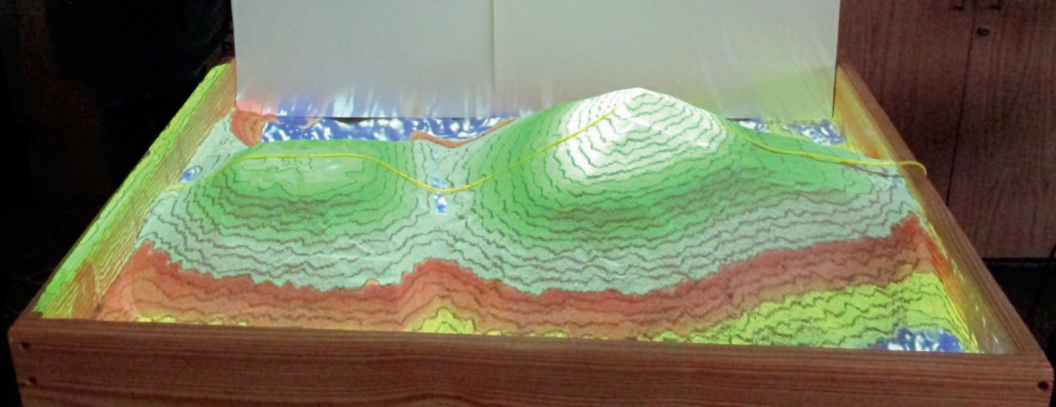
\includegraphics[width=0.9\linewidth]{figure/Analysis/augmentedrealitysandbox.png}
	\caption{Augmented reality sandbox showing a topographical map of the sand. Simulated water can be seen on the other side of the hill \cite{woods2016pilot}.}
	\label{fig:augmentedrealitysandbox}
\end{figure}


    
\subsection{Interactive Projection Mapping Prototype} % Daniel
    This project demonstrates the possibilities of manipulating the physical world using the Leap Motion in combination with an Arduino, as seen in \autoref{fig:leapProjector}. Using the Leap Motion API \todo{as described in section XYZ}, the creator allowed for simple gestures to control the box and pick up the pets in the world. The goal of the game is as simple as picking up the four pets and putting them on their pillow, all while rotation the cube to cycle through the different seasons and sides of the cube\cite{leapMotionProjectionMapping}.
    \begin{figure}[H]
    	\centering
    	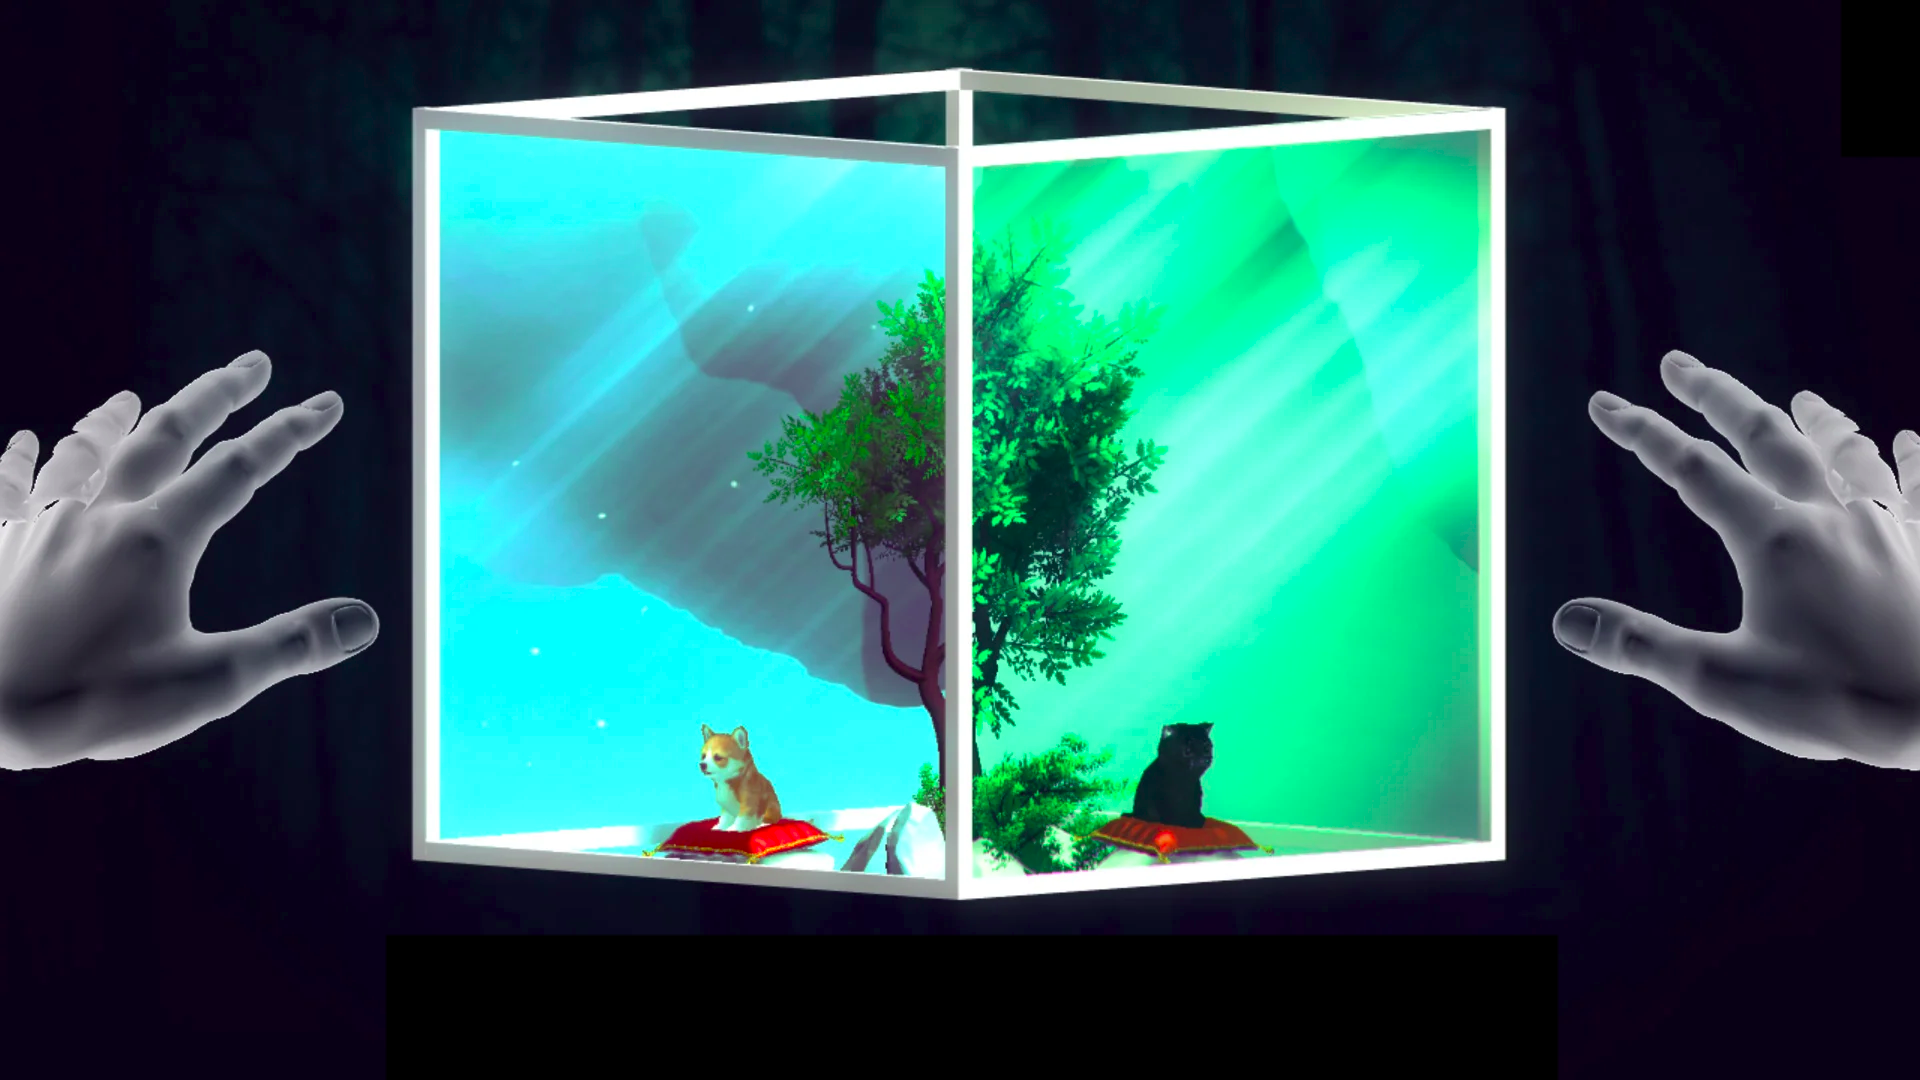
\includegraphics[width=0.8\linewidth]{figure/Analysis/LeapProjector.png}
    	\caption{A physical game, using the Leap Motion to pick up pets and rotating the physical cube using gestures\cite{leapMotionProjectionMapping}.}
    	\label{fig:leapProjector}
    \end{figure}
    The game can be played exclusively on the PC, without the physical cube. But the point from the creator's side was to learn to interface with the physical cube using the Leap Motion.
\subsection{Immersive Holodeck}\label{sec:leapMotionHolodeck} % Daniel
    A university in Ohio made an immersive \textit{"holodeck"} like experience, using 3 projectors in combination with a Leap Motion positioned in the the middle of the room. Using the leap motion, a user could manipulate objects in minecraft, like seen in \autoref{fig:holodeck}, or navigate around the world using Google maps\cite{leapMotionHolodeck}.
    
    \begin{figure}[H]
    	\centering
    	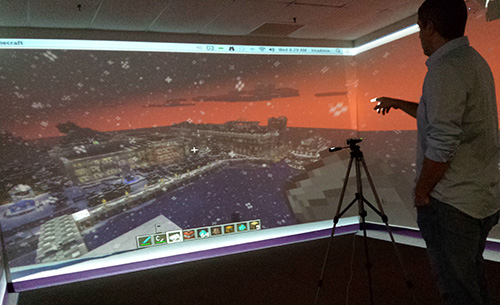
\includegraphics[width=0.7\linewidth]{figure/Analysis/holodeck.jpg}
    	\caption{Ohio university made immersive holodeck, made for immersive language learning\cite{leapMotionHolodeck}.}
    	\label{fig:holodeck}
    \end{figure}
    
    The purpose of the system, was to allow immersion while learning a language, putting you in the environments that the language is spoken.
\subsection{DybhavsVR} % Fredrik

\textbf{theBlu} is a virtual reality game developed by Wevr\footnote{https://blog.wevr.com/acclaimed-vr-series-theblu-out-on-transport-oculus-touch-896}. This game offers an immersive deep sea experience which puts the user in different environments under the ocean. The game offers three different undersea experiences. In the first experience, the user is placed on a boat and encounters a variety of species and in the end encounters a whale up close. There is no real control element in this experience and is solely an observation. The second experience is a Reef Migration, which the user will experience a variety of different reef animals such as turtles and different species of fish. As the first experience, this interaction does not offer controls either. The last experience is a Luminous Abyss experience, where the user will be enveloped in almost complete darkness, and then to be equipped with a flashlight utilizing tracked motion controllers to look around in the deep ocean. The user can then move around in a room scale while using the flashlight to illuminate different deep sea species around the vicinity. In \autoref{fig:theBlu} an example of the luminus abyss experience can be seen.
    \begin{figure}[H]
    	\centering
    	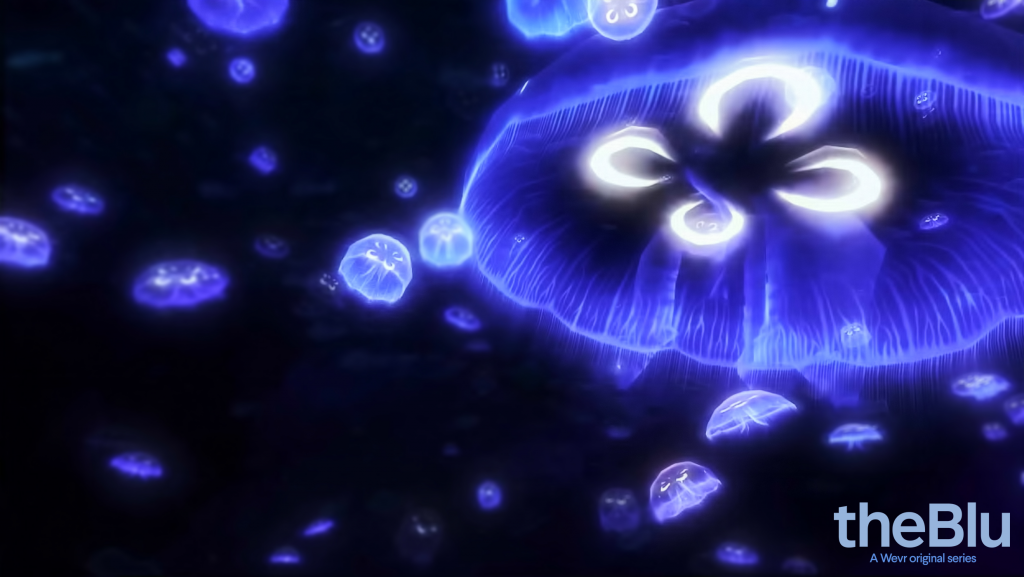
\includegraphics[width=0.9\linewidth]{figure/Analysis/theblu.png}
    	\caption{Wevr's theBlu game}
    	\label{fig:theBlu}
    \end{figure}
All these experiences can use a small room which offers the user to move around in a small vicinity while interacting with the experiences. 

\subsection{Transcending Boundaries}\label{sec:transcendingBoundaries} % Jens
Transcending Boundaries is an exhibition that ran in the beginning of 2017 at the Pace Gallery in London. It featured a series of immersive installations made by teamLab in an attempt to transcend the boundaries between digital artwork and the physical world\cite{transcendingBoundries}. \autoref{fig:transcendingBoundaries} shows a virtual waterfall, flowers and butterflies that are projected up on the walls and on the floor in one of the rooms of the exhibit using multiple projectors. The vegetation would indicate changes in seasons and would go through all 4 seasons every hour. Viewers in the room would obstruct the flow of water based on where they were standing and thereby became a part of the artwork. 

    \begin{figure}[H]
    	\centering
    	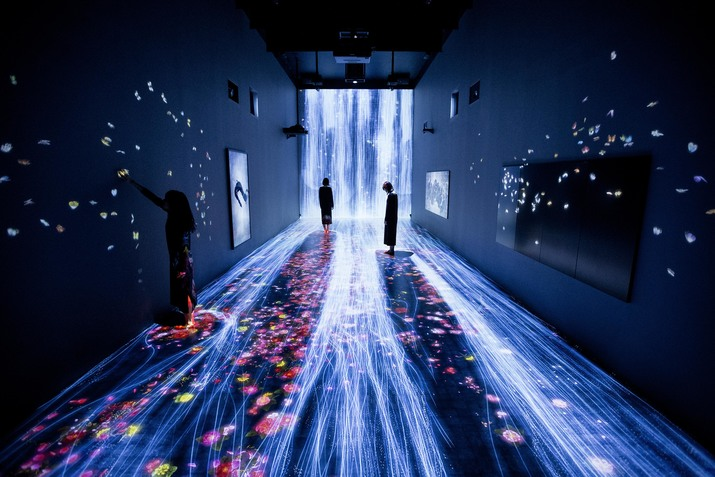
\includegraphics[width=0.9\linewidth]{figure/Analysis/transcendingBoundaries.jpg}
    	\caption{Figure showing 3 people interacting with the virtual waterfall installation from teamLab's exhibition at the Pace Gallery in London\cite{transcendingBoundries}.}
    	\label{fig:transcendingBoundaries}
    \end{figure}
    
\section{State of the Art - interaction/tracking Technology}
In the following sections the specifications, and application ideas for different technologies, will be presented in relation to possible ways of interacting with a projection.   
    
\subsection{The Nintendo Wii Remote } % Sofie
The Nintendo Wii Remote, is a controller designed for use with the Nintendo Wii console. It connects to the console with a short range Bluetooth connection with a maximum operating distance of approximately 10 meters\cite{WiimoteWIKI}\cite{WiimoteSpecs}. It features a built-in speaker, force feedback, and a motion sensor in form of an accelerometer, along with a optical censor, which is used to determine position and pointing direction by sensing light from a sensor bar connected to the console. The maximum measure distance for the optical sensor is 5 meters.\cite{WiimoteWIKI}. \\
These features might be used for this project, as a way of interacting with a installation. As inspiration for ways to do so, a project by the researcher Johnny Chung Lee \cite{JohnnyLeeWiiMoteDemo}, shows that the optical sensor of the Wii Remote can be used to interact with a projection, and to track head motion and viewing direction of a single user, in a simplistic manner. To do so, he uses the infrared senor in the Wii Remote, to act as a receiver, and a infrared LED as the device to be tracked by the Wii Remote. The Wii Remote is mounted to the screen/projection area, and the infrared LED(s) is provided to the user as integrated in a pen(infrared pen) or in glasses, depending on the wanted way of interaction. The software Lee uses, is open source and is designed to be used to create a low budged interactive whiteboard with the mentioned hardware (Wii Remote, infrared LED, and a screen/projector)\cite{JohnnyLeeWiiMProgram}.

\subsection{The Kinect for Xbox One (2013 version)}
The latest model of the Kinect, uses a time-of-flight camera, along with an infrared camera to track and read the environment\cite{KinectWiki}. The time-of-flight camera measures distance by emitting a pulse of light and then measure the time for the light signal to return in relation to the speed of light. Thereby calculating the distance to each point within the scene. 
This Kinect version can track within a 3 ft range, detect heart rate and facial expressions of the user, as well as estimate the joints and thereby skeletal composition of op to 6 users at the time\cite{KinectWiki}.\\
Part owner of an art collective named \textit{Floating Point} Jack Kalish \cite{LANscapes}, used the Kinect in an art installation \textit{LanScape}, where the users/observers movements would manipulate a digital landscape, projected on a wall. The landscape would or example take shape as mountains or valleys if the user would raise their arms or sit on the floor, respectively.  
Garratt Gallagher from MIT’s Computer Science and Artificial Intelligence Laboratory (CSAIL) \cite{MR_MIT}, used the Kinect to create an interface similar to the one seen in the fiction film \textit{Minority Report}. The Kinect can as seen, also be used to track gestures and thereby interact with interfaces. 


  

\subsection{Playstation DualShock 4 Controller}
The DualShock 4 is a wireless controller made by Sony for the Playstation 4(PS4). It features a touchpad, a 6-axis motion sensor(3-axis gyroscope and 3-axis accelerometer), a mono-speaker, various controls, lights and vibrations\cite{dualshock4}. When installing programs similar to DS4Windows\footnote{DS4Windows website: \url{http://ds4windows.com/}} on a PC it is possible to connect the DualShock4 to the PC and thereby take advantage of its features on this platform.

\subsection{Leap Motion} % Daniel
    Leap motion is a tool that is used for tracking hands and fingers in real time\cite{leapMotion}. The newest iteration integrates with Virtual Reality, hence eliminating the need for having a controller in your hand. The Leap Motion controller functions by having three IR LEDs and two monochromatic IR Cameras. The maximum reading distance from the controller is approximately 1m\cite{leapMotion}. The accuracy of the controller is roughly 0.7mm, hence the virtual version of ones hands can be very precise as seen in \autoref{fig:leapMotion}.
    
    \begin{figure}[H]
    	\centering
    	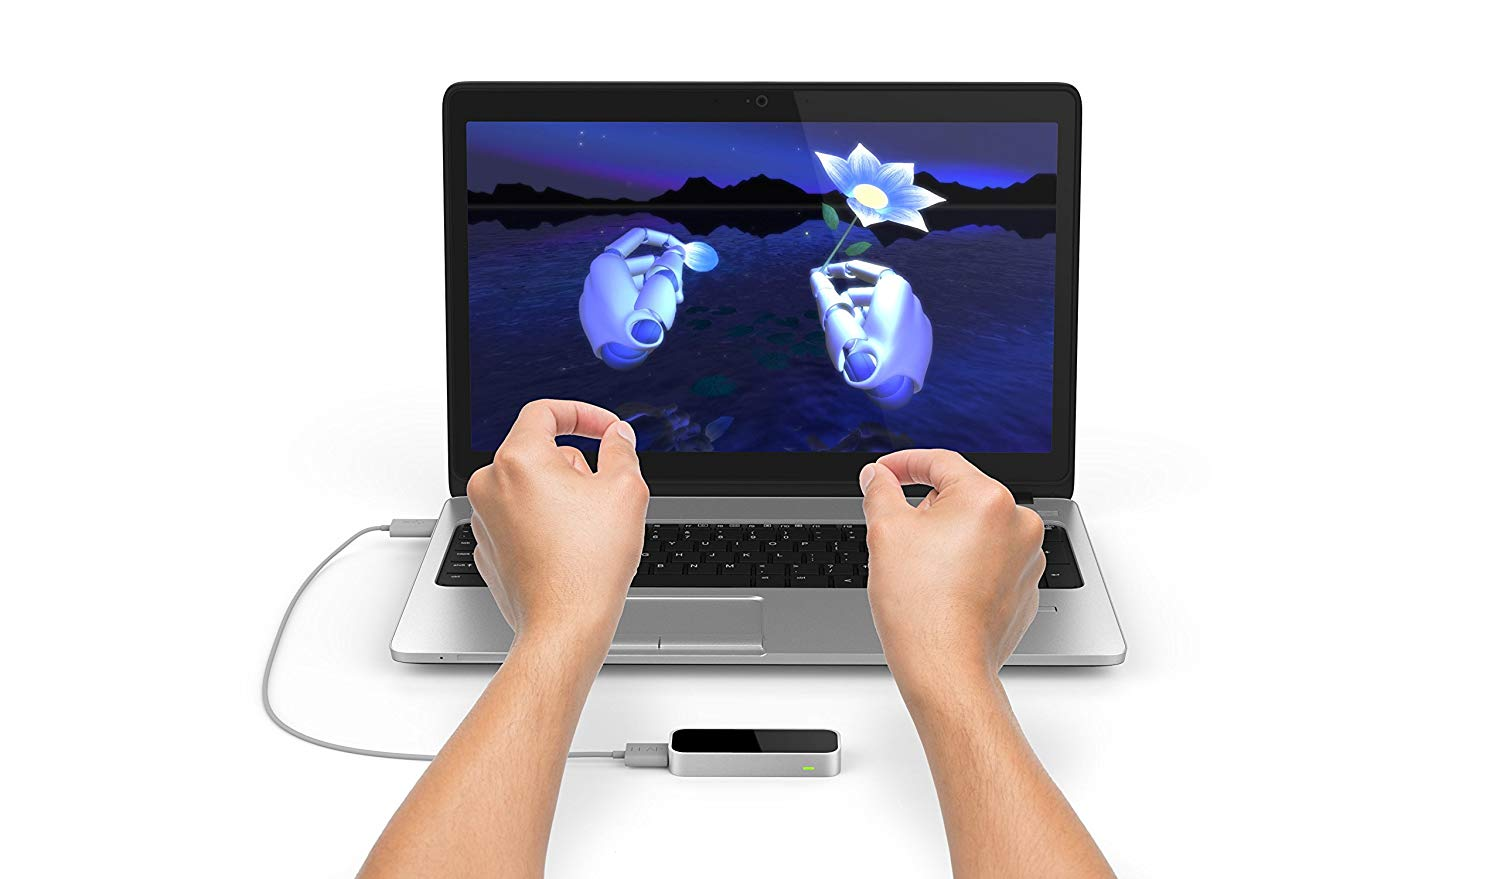
\includegraphics[width=0.9\linewidth]{figure/Analysis/leapMotion.jpg}
    	\caption{Image of the Leap Motion in action, taken from the Amazon store page.}
    	\label{fig:leapMotion}
    \end{figure}

\subsection{Multiple Display setups}
As seen in \autoref{sec:leapMotionHolodeck} and \autoref{sec:transcendingBoundaries} multiple projectors working in tandem are utilized to create immersive technology. There are several ways of having multiple projectors working together. Using a Graphical Processing Unit, or GPU for short with sufficient outputs to drive all the required projectors. Newer graphics cards can run up to 4 monitors at the same time \footnote{GTX 1080TI: \url{https://www.evga.com/products/product.aspx?pn=11G-P4-6693-K3}}, or with the use of a display port hub, splitting the bandwidth of the display ports to allow more monitors at lower resolutions\footnote{EVGA DisplayPort Hub\url{https://www.evga.com/products/product.aspx?pn=200-dp-1301-l1}} which makes it possible to run even more screens off a single high end GPU, depending on how many display ports it has. If more monitors than this are needed, multiple GPU's can be installed in the same system, and even more displays can be used. Another way to achieve multiple displays with a single display port is using a technology called daisy chaining. The principle behind this is to connect multiple displays supporting display ports where each one is connected in sequence to each other, hence only requiring one output from the GPU. Depending on the resolution this can be done with 2-5 monitors\cite{displayport}.

\section{Perception}
% https://ieeexplore.ieee.org/document/1667620/#full-text-section

% https://link.springer.com/article/10.1007/BF00896880

% file:///Users/damh/Downloads/927-3572-1-SM.pdf

% http://diposit.ub.edu/dspace/bitstream/2445/49643/1/631349.pdf



\section{Gamification}
    The definition of gamification this paper is adhering to is defined by Sebastian Deterdin et al as being: \begin{quote}
        \textit{"the use of game design elements in non-game contexts"}\cite{gamification}.\\
    \end{quote}
    The paper tries to define gamification due to the popularity the word has gotten in both the industry and scientific space\cite{gamification}.